 \providecommand{\main}{../../..}
\documentclass[\main/main.tex]{subfiles}
\begin{document}
\subsection{Esercizio 1}
Dato il seguente problema di PL:

\begin{figure}
  \begin{align*}
    \max z = 2x_1 + x_2    \\
    3x_1 + 4x_2  & \leq 12 \\
    x_1 + x_2    & \geq 1  \\
    -9x_1 + 4x_2 & \leq 0  \\
    3x_1 - 8x_2  & \leq 3  \\
    x_1, x_2     & \geq 0
  \end{align*}
  \caption{Esercizio 1}
\end{figure}

\begin{enumerate}
  \item Si disegni la regione ammissibile e si evidenzi il vertice ottimo per via grafica, riportando il valore di z e di tutte le variabili del modello, comprese quelle di scarto.
  \item Da quali variabili è composta la base associata al vertice dato dall'intersezione del secondo e terzo vincolo?
  \item Si ricavi per via grafica per quali valori di $b_4$, ora pari a $3$, la \textbf{composizione} della base ottima non cambia.
  \item Si risolva mediante gli scarti complementari il duale del problema.
\end{enumerate}

\subsection{Soluzione esercizio 1}

\subsubsection*{Identifico soluzione ottima}

\begin{figure}
  \begin{subfigure}{0.49\textwidth}
    \dddgraph{x_1}{x_2}{0}{3}{0}{2.5}{0}{
      3*x + 4*y  <= 12 &&
      x + y    >= 1  &&
      -9*x + 4*y <= 0  &&
      3*x - 8*y  <= 3
    }{2*x +y}
    \caption{Il vertice ottimo ha coordinate $\bmx = \rnd{3,\frac{3}{4}}$}
  \end{subfigure}
  \begin{subfigure}{0.49\textwidth}
    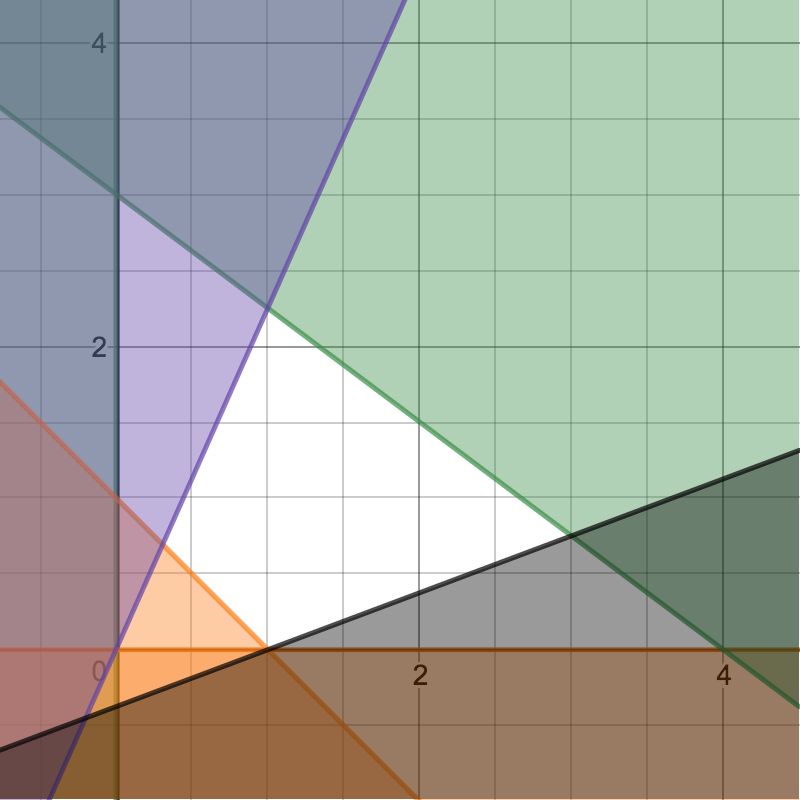
\includegraphics[width=0.9\textwidth]{2015_09_16}
    \caption{Regione di ammissibilità del problema}
  \end{subfigure}
  \caption{Vertice ottimo del problema di minimo}
\end{figure}

\subsubsection*{Riporto variabili}

\begin{align*}
  z   = \frac{27}{4}, \quad
  x_1 = 3           , \quad
  x_2 = \frac{3}{4} , \quad
  s_1 = 0           , \quad
  s_2 = \frac{11}{4}, \quad
  s_3 = 24          , \quad
  s_4 = 0
\end{align*}
\subsubsection*{Variabili di base}
TODO: mi verrebbe istintivo dire $x_1$ e $x_2$.

\subsubsection*{Analisi di sensitività}
Il valore di $b_4$ può variare tra $-15$ e $12$.

\begin{figure}
  \begin{subfigure}{0.49\textwidth}
    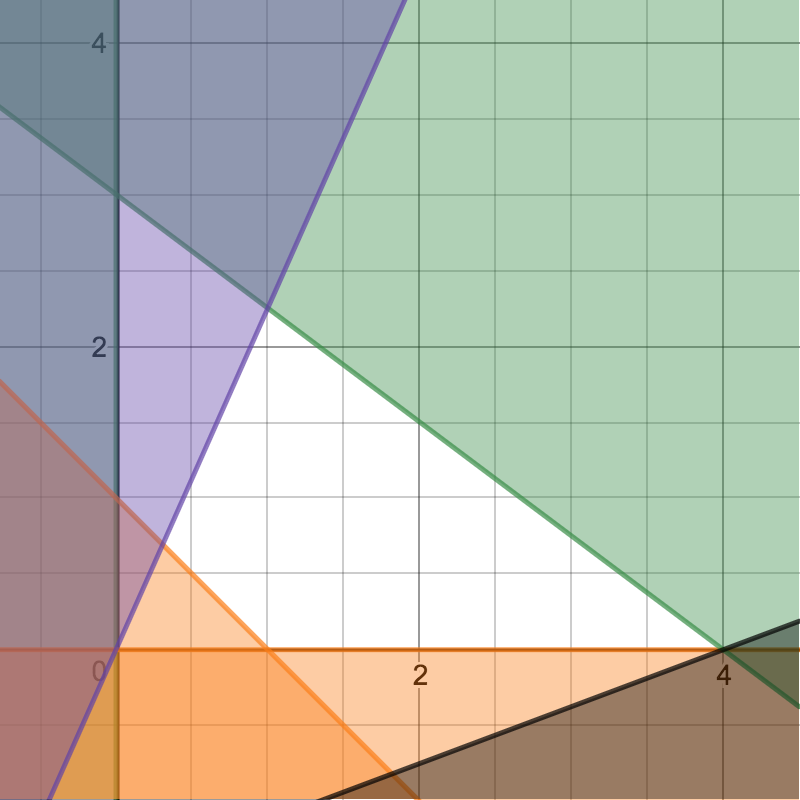
\includegraphics[width=0.9\textwidth]{2015_09_16_1}
    \caption{$3(4)-8(0)= b_4 = -15$}
  \end{subfigure}
  \begin{subfigure}{0.49\textwidth}
    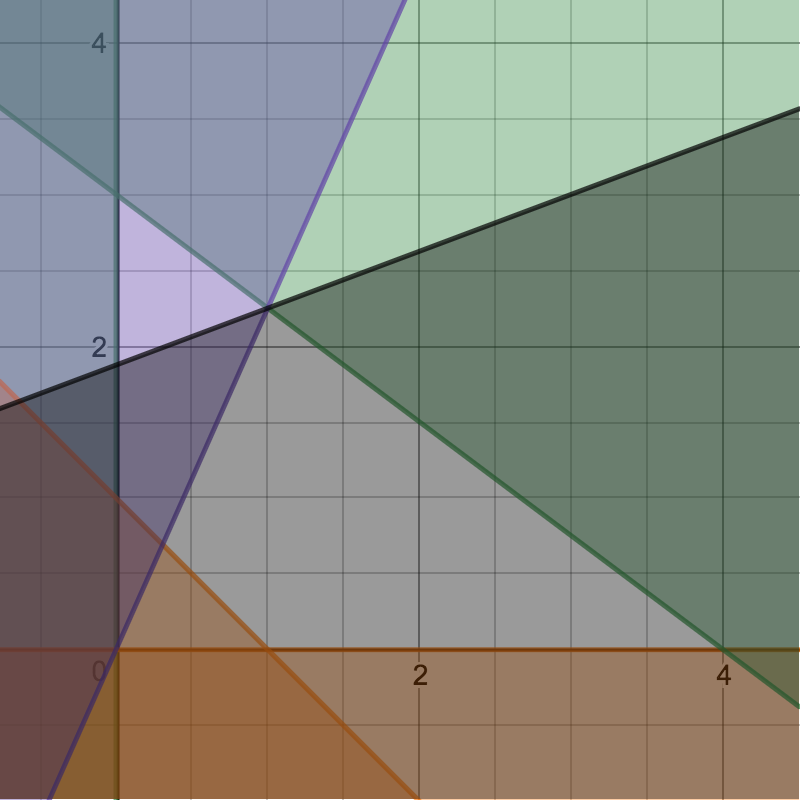
\includegraphics[width=0.9\textwidth]{2015_09_16_2}
    \caption{$3(1)-8(2.25)= b_4 = 12$}
  \end{subfigure}
  \caption{Analisi di sensitività}
\end{figure}

\subsubsection*{Costruisco problema duale}
\begin{align*}
  \min z_D = 12y_1 + y_2 + 3y_4    \\
  3y_1 + y_2 - 9y_3 +3y_4 & \geq 2 \\
  4y_1 + y_2 + 4y_3 -8y_4 & \geq 1 \\
  y_1, y_3, y_4           & \geq 0 \\
  y_2                     & \leq 0
\end{align*}
\subsubsection*{Scarti complementari}
\[
  \begin{cases}
    x_1(3y_1 + y_2 - 9y_3 +3y_4 -2) = 0 \\
    x_2(4y_1 + y_2 + 4y_3 -8y_4 -1) = 0 \\
    y_1(3x_1 + 4x_2  -12) = 0           \\
    y_2(x_1 + x_2    -1 ) = 0           \\
    y_3(-9x_1 + 4x_2 -0 ) = 0           \\
    y_4(3x_1 - 8x_2  -3 ) = 0           \\
  \end{cases}
  \Rightarrow
  \begin{cases}
    3y_1 +3y_4 -2 = 0 \\
    4y_1 -8y_4 -1 = 0 \\
    y_2 = 0           \\
    y_3 = 0           \\
  \end{cases}
  \Rightarrow
  \begin{cases}
    y_1 = \frac{2}{3} -y_4               \\
    4\rnd{\frac{2}{3} -y_4} -8y_4 -1 = 0 \\
    y_2 = 0                              \\
    y_3 = 0                              \\
  \end{cases}
  \Rightarrow
  \begin{cases}
    y_1 = \frac{19}{36} \\
    y_4 = \frac{5}{36}  \\
    y_2 = 0             \\
    y_3 = 0             \\
  \end{cases}
\]
Le soluzioni ottime coincidono: $z = z_D = \frac{27}{4}$.
\end{document}